\section{Análise e pré-processamento dos dados}
Para a análise do nosso problema, não seria pertinente estudar as palavras separadamente, pois não há sentido semântico. Decidimos então utilizar as letras, sem pontuação, sem espaçamento e sem dígitos.

Os caracteres especiais, como letras acentuadas, podes ser consideradas como cruciais para a predição, mas elas servem como forma de ruído, já que nomes de pessoas e de lugares podem aparecer em ambos os tipos de texto.

A quantidade de cada caractere é uma informação relevante, mas não podendo ser utilizada crua, pois se analisarmos um texto com o total de 500 caracteres em inglês que contém 50 letras “a”, não pode ser considerado em potuguês por causa da distância dele com um outro texto de 100 caracteres que comtém 50 letras “a” ser pequena. Por esses motivos, sentimos a necessidade de usar a porcentagem de ocorrência cada letra no texto.

No exemplo a seguir, temos dois textos e seus histogramas, para melhor visualisação dos dados utilizados.

\begin{framed}
    \texttt{Perceived end knowledge certainly day sweetness why cordially. Ask quick six seven offer see among. Handsome met debating sir dwelling age material. As style lived he worse dried. Offered related so visitor we private removed. Moderate do subjects to distance.\\Of friendship on inhabiting diminution discovered as. Did friendly eat breeding building few nor. Object he barton no effect played valley afford. Period so to oppose we little seeing or branch. Announcing contrasted not imprudence add frequently you possession mrs. Period saw his houses square and misery.}
\end{framed}
\captionof{figure}{Texto do Random Text Generator~\cite{site:rtg}}

\begin{framed}
    \texttt{Ainda assim, existem dúvidas a respeito de como a execução dos pontos do programa facilita a criação das direções preferenciais no sentido do progresso. Por outro lado, o novo modelo estrutural aqui preconizado cumpre um papel essencial na formulação das novas proposições.\\O empenho em analisar o consenso sobre a necessidade de qualificação exige a precisão e a definição dos relacionamentos verticais entre as hierarquias. Todas estas questões, devidamente ponderadas, levantam dúvidas sobre se a revolução dos costumes deve passar por modificações a longo prazo.}
\end{framed}
\captionof{figure}{Texto do Lero Lero~\cite{site:lero}}

\begin{center}
    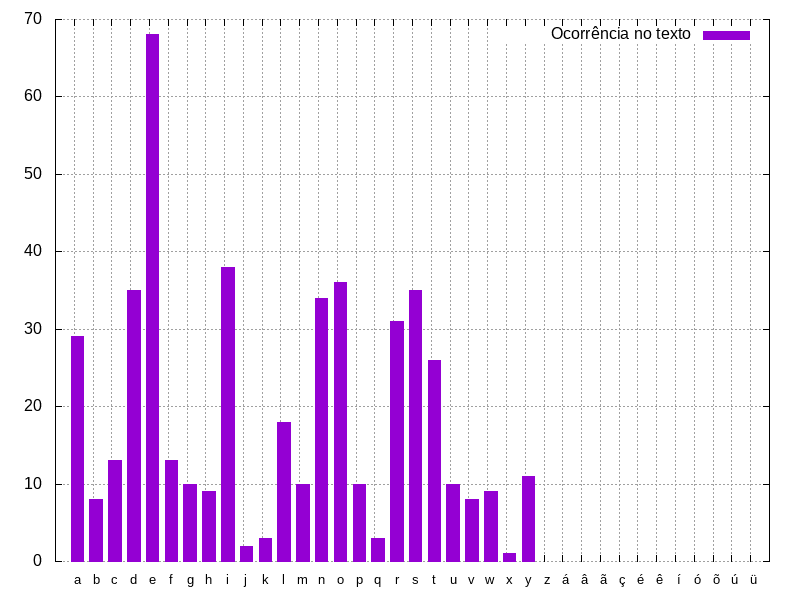
\includegraphics[width=0.8\linewidth]{freq-en.png}
    \captionof{figure}{Histograma do texto em inglês}
\end{center}

\begin{center}
    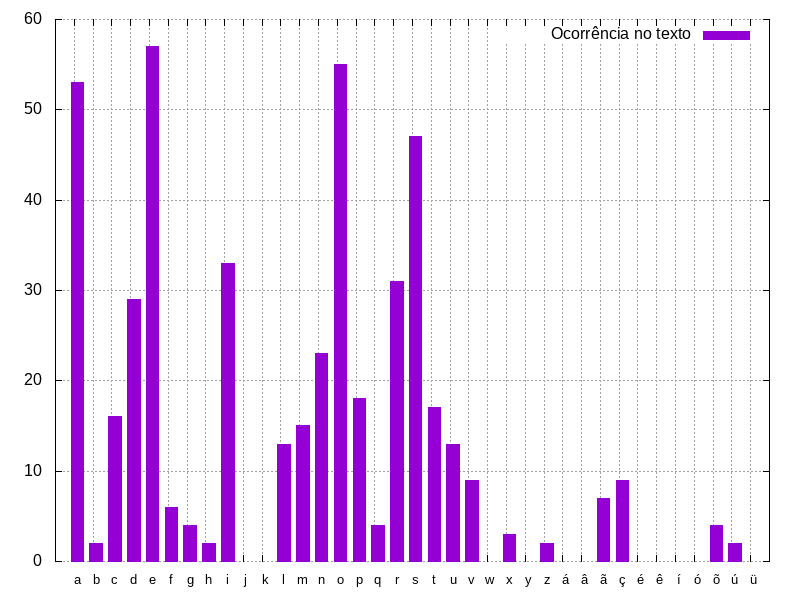
\includegraphics[width=0.8\linewidth]{freq-ptbr.png}
    \captionof{figure}{Histograma do texto em português}
\end{center}
